\documentclass{article}


\usepackage{PRIMEarxiv}

\usepackage[utf8]{inputenc} % allow utf-8 input
\usepackage[T1]{fontenc}    % use 8-bit T1 fonts
\usepackage{hyperref}       % hyperlinks
\usepackage{url}            % simple URL typesetting
\usepackage{booktabs}       % professional-quality tables
\usepackage{amsfonts}       % blackboard math symbols
\usepackage{nicefrac}       % compact symbols for 1/2, etc.
\usepackage{microtype}      % microtypography
\usepackage{lipsum}
\usepackage{fancyhdr}       % header
\usepackage{graphicx}       % graphics
\graphicspath{{media/}}     % organize your images and other figures under media/ folder


% stuff Spencer added
\usepackage{amsthm} % for proof and theorem environments
\usepackage{amsmath} % for math text

\newtheorem{theorem}{Theorem}[section]
%Header
\pagestyle{fancy}
\thispagestyle{empty}
\rhead{ \textit{ }} 

% Update your Headers here
\fancyhead[LO]{Running Title for Header}
% \fancyhead[RE]{Firstauthor and Secondauthor} % Firstauthor et al. if more than 2 - must use \documentclass[twoside]{article}



  
%% Title
\title{A template for Arxiv Style
%%%% Cite as
%%%% Update your official citation here when published 
\thanks{\textit{\underline{Citation}}: 
\textbf{Authors. Title. Pages.... DOI:000000/11111.}} 
}

\author{
  Author1, Author2 \\
  Affiliation \\
  Univ \\
  City\\
  \texttt{\{Author1, Author2\}email@email} \\
  %% examples of more authors
   \And
  Author3 \\
  Affiliation \\
  Univ \\
  City\\
  \texttt{email@email} \\
  %% \AND
  %% Coauthor \\
  %% Affiliation \\
  %% Address \\
  %% \texttt{email} \\
  %% \And
  %% Coauthor \\
  %% Affiliation \\
  %% Address \\
  %% \texttt{email} \\
  %% \And
  %% Coauthor \\
  %% Affiliation \\
  %% Address \\
  %% \texttt{email} \\
}


\begin{document}
\maketitle


\begin{abstract}
Detecting shared neural activity across individuals experiencing the same 
naturalistic stimulus can reveal stimulus-driven brain responses, inform on 
brain regions' 
functional roles, and identify potential clinical biomarkers.
Intersubject correlation (ISC) includes the primary methods
for detecting voxelwise 
regions of shared response and quantifying subject-level variability.
However, ISC analyses require thousands of voxelwise tests, leading to 
multiple-comparison problems, and even nonparametric resampling methods 
often produce liberal sampling distribution which inflate false positives.
ISC methods treat voxels independently and lack 
principled ways to incorporate spatial structure.
We propose a model-based alternative to ISC that simultaneously estimates the 
shared neural response function and spatial activation patterns using a 
Gaussian process framework coupled with a Bayesian spatial sparsity prior 
inspired by the horseshoe prior.
We examine the properties of this prior—designed to induce stronger shrinkage 
than the standard horseshoe—and evaluate the model’s performance in simulations 
and real fMRI data.
The Bayesian model provides natural uncertainty quantification of the 
shared response function, and in the analyses it demonstrates better control 
of false positives 
relative to ISC approaches.
\end{abstract}


% keywords can be removed
\keywords{First keyword \and Second keyword \and More}

\section{Introduction}

\begin{itemize}
  \item Intersubject correlation theory
  \item ISC estimation methods
  \begin{itemize}
    \item Testing is weak
    \item Cannot estimate function with uncertainty
  \end{itemize}
  \item Estimate function with uncertainty using GP
  \item Use horseshoe prior for ARD voxel activation
  \item Introduce data
\end{itemize}


\section{Methodology}

The overall model which is used is in equation \ref{eq:overall_model}. Here
$B_{s,v} (t)$ is the bold response for subject $s$ voxel/location $v$ at time
$t$. Together $\beta_v$ and $f(t)$ capture the shared signal $c(t)$ from 
\cite{nastase2019measuring}. The parameter $\beta_v$ determines how much of the
signal is explained by the shared latent function $f(t)$. 
A major purpose of this
paper is to model $\beta_v$ such that it indicates for each voxel whether or 
not the shared function $f(t)$. The error term $\epsilon_{s,v}(t)$ follows an 
autoregressive of lag 1 process. The autoregressive coefficient $\gamma_v$
and the variance parameter $\sigma^2_{\eta v}$ are shared among subjects. It
may be preferable that they not be shared among subjects, but this decision
follows with what others have done in the literature \cite{mejia2020bayesian}.
More importantly, having a 
separate parameter for each subject gives a huge number of parameters and
makes computation far more intense. If inference on the idiosynchratic functions
for each subject is particularly important, one may fit the model in 
\ref{eq:overall_model} where the errors are independent. Then after fitting
the overall model, the residuals can be calculated as 
$\widehat{\beta_v f(t)} - B_{s,v}$ and the residuals for each subject could be 
analyzed.

A contribution of this paper is to estimate $f(t)$ in the scenario where 
subjects are exposed to natural stimuli. However, if task based experimation
is performed, $f(t)$ may be the hemodynamic response function convolved with 
the task, making model the task based general linear model a special case of
$\ref{eq:overall_model}$ where there is only 1 task.

\begin{equation}
  \begin{aligned}
    B_{s,v} (t) &= \beta_{v} f(t) + \epsilon_{s,v}(t) \\
    \epsilon_{s,v} (t) &= \gamma_v \epsilon_{s,v} (t - 1) + \eta_{s,v} \\
    \eta_{s,v} &\sim N(0, \sigma^2_{\eta v})
  \end{aligned}
  \label{eq:overall_model}
\end{equation}


The prior distribution on $\beta_v$ is very similar to the horseshoe prior
\cite{carvalho2009handling,carvalho2010horseshoe}. However, the heavy tails
on the horshoe prior led to higher false discovery rates of activated voxels. 
Thus in \ref{eq:hs_prior}, the parameter $\lambda_v$ is given a half-normal
component as opposed to half-Cauchy component in the horseshoe. This makes the
tails lighter and provides more shrinkage. The paper 
\cite{bhadra2017horseshoe+} is not of direct importance to the prior I use here,
but it led me to explore some theoretical results of the prior I use, most 
notably the infinite spike at 0. It was the exploration of that property which 
led me to recognize the marginal distribution of the prior I'm using as a 
function of the Matern type 2. \cite{piironen2017hyperpriora} and 
\cite{piironen2017sparsityb} provide a principled approach for selecting the
hyperprior on the global shrinkage parameter $\tau$. They use some theory from
a different paper, and that suggestion is roughly though not 
exactly followed in this paper. Following that rough construction, 
we set $\tau_0 = .1/\sqrt{S\times V \times T}$. Another modification is to use
here a half-normal distribution instead of a half-Cauchy distribution. 

The activation of a voxel will naturally be related to the surrounding voxels,
so it makes sense to borrow spatial information. This is done by modeling the 
scale parameter of the prior on $\lambda_v$ according to a spatial process. 
Because of its speed in fitting, we model $\boldsymbol{\alpha}$ according to
an intrinsic conditional autoregressive (ICAR) model \cite{besag1974spatial}.
I use four neighbors, which is called the nearest neighbor approach 
\cite{besag1974}.


\begin{equation}
  \begin{aligned}
    \beta_v | \lambda_v, \tau &\sim N^+(0, \lambda_v^2 \tau^2) \\
    \lambda_v | \phi_v &\sim N^+(0, \phi_v^2) \\
    \tau &\sim N^+(0, \tau_0^2)
    \end{aligned}
  \label{eq:hs_prior}
\end{equation}



\begin{equation}
  \begin{aligned}
    \phi_v &= \text{logit} (\alpha_v) \\
    \alpha_v | \alpha_{v \sim v'} &\sim
            N\left(\frac{\sum_{v \sim v'} \alpha_i}{d_i},
                   \frac{1}{d_i}\right)
  \end{aligned}
  \label{eq:icar1}
\end{equation}

\begin{equation}
  p(\boldsymbol{\alpha}) \propto \text{exp} \left(-\frac{1}{2} \sum _{v \sim v'}
      (\alpha_v - \alpha_{v'})^2 \right)
  \label{eq:icar1}
\end{equation}




\section*{Normal horseshoe}

\[
 p(\kappa | \tau) = \frac{1}{\tau} \frac{1}{\sqrt{2 \pi} \kappa^{3/2} \sqrt{1 - \kappa}}
 \text{exp} \left(-\frac{(1-\kappa)}{2 \kappa \tau^2} \right)
\]



The prior distribution used to 

\begin{theorem}
For $\tau = 1$, the marginal density of the ?? prior satisfies the following
properties:

\begin{enumerate}
\item
\[
  \pi (\theta) = \frac{1}{\pi}K_0(|\theta|)
\]

where $K_0(\cdot)$ is the modified Bessel function of the second kind.

\item
\[
     \lim_{|\theta| \to 0} \pi (\theta) = \infty
\]
\end{enumerate}
\end{theorem}

\begin{proof}
\[
  p(\theta) = \int_0^{\infty} 
              \frac{1}{\sqrt{2 \pi \lambda^2}} 
              \text{exp}\left(-\frac{\theta^2}{2 \lambda ^2} \right)
              \sqrt{\frac{2}{\pi}}
              \text{exp}\left(-\frac{- \lambda^2}{2} \right) d\lambda
\]

Apply the transformation $\zeta = \lambda^2 / 2$ to get

\begin{align*}
&= \frac{1}{2\pi} \int_0^{\infty} \frac{1}{\zeta} \text{exp} 
              \left(-\zeta -\frac{\theta}{4 \zeta} \right) d\zeta \\
          &= \frac{1}{\pi}K_0(|\theta|)
\end{align*}
where $K_0(\cdot)$ is the modified Bessel function of the second kind. This 
relationship between the preceeding functions is seen in 10.32.10 of
\cite{olver2010nist}. As $|\theta| \rightarrow 0$, 
$K_0(|\theta|) \rightarrow \infty$.


\end{proof}


\begin{figure}[hbt!]
    \centering
    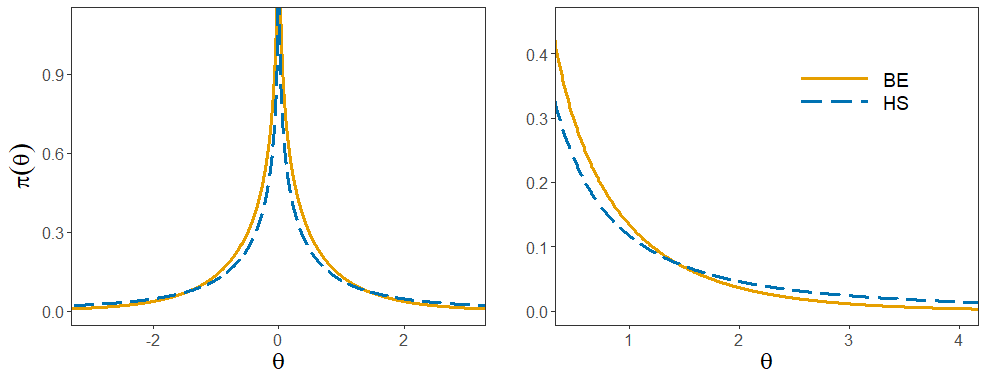
\includegraphics[scale=.55]{images/marg_priors.png}
    \caption{}
    \label{fig:marg_priors}
\end{figure}

\begin{figure}[hbt!]
    \centering
    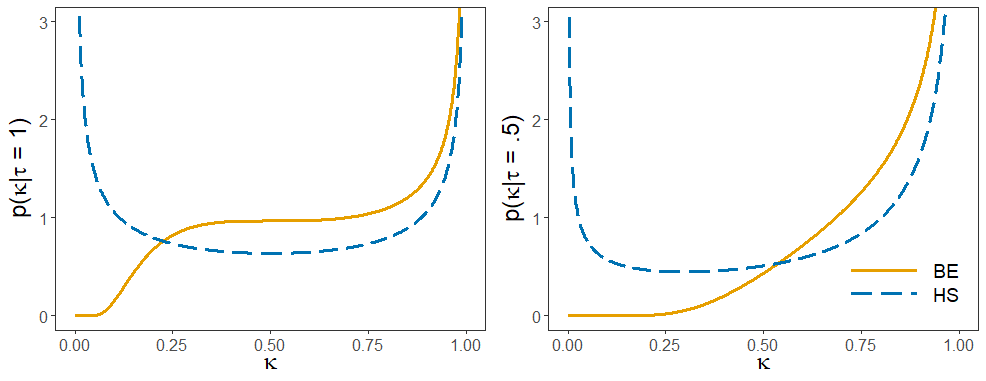
\includegraphics[scale=.55]{images/kappa_priors.png}
    \caption{}
    \label{fig:marg_priors}
\end{figure}


\begin{itemize}
  \item GP regression
  \begin{itemize}
    \item Nearest neighbor GP regression
    \item Automatic relevance determination
  \end{itemize}
  \item Horseshoe prior
  \item Full model methodolgy
  \begin{itemize}
    \item Prior distribution selection
    \item Spatial prior and independent prior
  \end{itemize}
  \item Stan implementation
\end{itemize}

\section{Simulation}
\begin{itemize}
  \item Simulate via neurosim
  \item Compare ISC methods, independent and spatial priors
  \begin{itemize}
    \item Voxel activation
    \begin{itemize}
      \item Precision
      \item Recall
    \end{itemize}
    \item Function estimation
  \end{itemize}
\end{itemize}

\section{Real data analysis}
\begin{itemize}
  \item Data details
  \item Redo simulation
  \item Analysis results
\end{itemize}

\section{Conclusion}
\begin{itemize}
  \item Accurate activation detection
  \item Allows for uncertainty in function
  \item Horsehoe metrics hand wavy
  \item Is not time specific
  \item Limited to ISC, not 
  \item Extend to multi-output GP
\end{itemize}

\section{Appendix}




\begin{theorem}
\[
  K \frac{1}{2}\text{exp} \left(-\frac{\theta^2}{4}\right)
    \text{log}\left(1 + \frac{8}{\theta^2}\right)
\]
\end{theorem}
\begin{proof}
\[
  p(\theta) = \int_0^{\infty} 
              \frac{1}{\sqrt{2 \pi \lambda^2}} 
              \text{exp}\left(-\frac{\theta^2}{2 \lambda ^2} \right)
              \sqrt{\frac{2}{\pi}}
              \text{exp}\left(-\frac{- \lambda^2}{2} \right) d\lambda
\]

Apply the transformation $\zeta = 2/ \lambda^2$ to get

\[
\begin{aligned}
  p(\theta) &= \frac{1}{2\pi} \int_0^{-\infty} \frac{1}{\zeta}
              \text{exp} \left(-\frac{\theta^2}{4}\zeta \right)
              \text{exp} \left(-\frac{1}{\zeta} \right) d\zeta \\
            &\geq K \int{1}{\infty} \frac{1}{\zeta}
              \text{exp} \left(-\frac{\theta^2}{4} \zeta\right) d\zeta \\
            &= K E_1 \left(\frac{\theta^2}{4} \right)
\end{aligned}  
\]
where $K = (2 \pi)^{-1} \text{exp}(-1)$ and $E_1(\cdot)$ is the exponential
integral function. This function satisfies the lower and upper bounds
\[
  \frac{\text{exp}(-t)}{2} < \text{log} \left(1 + \frac{2}{t}\right) <
  E_1(t) < \text{exp}(-t) \text{log} \left(1 + \frac{1}{t}\right)
\]
\end{proof}
%Bibliography
\bibliographystyle{unsrt}  
\bibliography{references}  


\end{document}
